\documentclass[11pt,a4paper]{article}

\usepackage[margin=2.6cm]{geometry}
\usepackage{amsmath,amssymb}
\usepackage{booktabs}
\usepackage{tikz}
\usepackage{xcolor}
\usepackage[colorlinks=true,linkcolor=blue!55!black,urlcolor=blue!55!black]{hyperref}
\usetikzlibrary{positioning,fit,backgrounds,arrows.meta,decorations.pathreplacing,patterns}

\newcommand{\Sop}{\hat{S}}
\newcommand{\code}[1]{\texttt{\small #1}}

\title{The single-spin (Option~2) preconditioner in SBD/gdb:\\
what was wrong and what changed}
\author{}
\date{2026--08--17}

\begin{document}
\maketitle

\begin{abstract}
\noindent
The projected (single-spin) Davidson solver in \code{gdb} converged to
energies \emph{above} the true root, with the discrepancy growing with the
size of the projected space, while the spin of every converged root remained
exactly correct. This note documents the cause --- the preconditioner used
only the determinant-diagonal part of the projected Hamiltonian, silently
discarding the intra-configuration exchange elements --- and the fix, which
builds the exact block diagonal of $V^{\mathsf T} H V$. Convergence became
monotone and the iteration count at $K=113\,394$ dropped from a stall to
25~matrix--vector products. Commit \code{f0ff1b8}.
\end{abstract}

\section{Setting}

Option~2 produces wavefunctions of a single total spin $S$ by projecting the
(Anderson spin-completed) determinant space onto the target-$S$ CSF space
\emph{before} diagonalising. Let

\begin{itemize}\itemsep2pt
  \item $H$ be the Hamiltonian in the determinant basis, of dimension
        $N_{\text{det}}$;
  \item $V$ be the determinant$\,\to\,$CSF map, of shape
        $N_{\text{det}}\times K$, with $K$ the number of target-$S$ CSFs.
\end{itemize}

$V$ is block diagonal by spatial configuration. Because $\Sop^2$ does not mix
different spatial configurations, each block can be built independently: for a
configuration with $n_{\text{open}}$ singly occupied orbitals one enumerates
its $Sz$-preserving spin arrangements, diagonalises the small canonical
$\Sop^2$ matrix, and keeps the eigenvectors with eigenvalue
$S(S+1)$. Blocks are cached by $n_{\text{open}}$, since the canonical
$\Sop^2$ block does not depend on which orbitals are involved.

The solver then runs a block Davidson--Liu iteration on the projected operator

\begin{equation}
  \tilde H \;=\; V^{\mathsf T} H V ,
  \label{eq:proj}
\end{equation}

applied matrix-free as
$x_{\text{csf}} \to V x_{\text{csf}} \to H(\cdot) \to V^{\mathsf T}(\cdot)$.
Every iterate is a combination of target-$S$ CSFs, so spin purity is
structural: it holds for any preconditioner, however bad.

\begin{figure}[t]
\centering
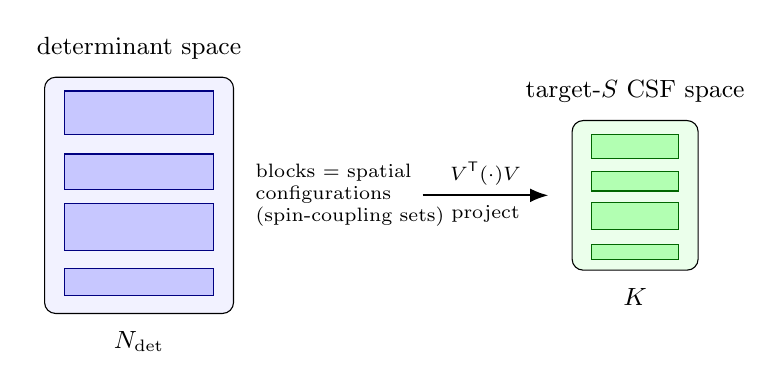
\begin{tikzpicture}[font=\small,>=Latex]

  % determinant space
  \node[draw,rounded corners,minimum width=2.4cm,minimum height=3.0cm,
        fill=blue!5] (det) at (0,0) {};
  \node[above=1mm of det] {determinant space};
  \node[below=1mm of det] {$N_{\text{det}}$};

  % blocks inside det space
  \foreach \y/\h in {1.05/0.55, 0.30/0.45, -0.40/0.6, -1.10/0.35} {
    \draw[fill=blue!22,draw=blue!50!black]
      (-0.95,\y-\h/2) rectangle (0.95,\y+\h/2);
  }
  \node[right=0.15cm of det,align=left,text width=2.4cm,font=\scriptsize]
    {blocks = spatial\\configurations\\(spin-coupling sets)};

  % arrow
  \draw[->,thick] (3.6,0) -- node[above,font=\scriptsize]{$V^{\mathsf T}(\cdot)V$}
                            node[below,font=\scriptsize]{project} (5.2,0);

  % csf space
  \node[draw,rounded corners,minimum width=1.6cm,minimum height=1.9cm,
        fill=green!8] (csf) at (6.3,0) {};
  \node[above=1mm of csf] {target-$S$ CSF space};
  \node[below=1mm of csf] {$K$};
  \foreach \y/\h in {0.62/0.3, 0.18/0.25, -0.26/0.34, -0.72/0.2} {
    \draw[fill=green!30,draw=green!40!black]
      (5.75,\y-\h/2) rectangle (6.85,\y+\h/2);
  }

\end{tikzpicture}
\caption{Option~2 in one picture. $V$ is block diagonal by spatial
configuration; each block is one spin-coupling set. The projection keeps only
the target-$S$ columns, so $K < N_{\text{det}}$ and every iterate is
single-$S$ by construction.}
\label{fig:projection}
\end{figure}

\section{The defect}

Davidson needs a cheap approximation to the diagonal of the operator it is
solving, used to precondition the residual:

\begin{equation}
  t_i \;=\; \frac{r_i}{E^{(p)} - D_i},
  \qquad D_i \approx \tilde H_{ii}.
  \label{eq:precond}
\end{equation}

The original code computed, for CSF column $c$ of a block,

\begin{equation}
  D_c^{\text{old}} \;=\; \sum_{r} V_{rc}^{2}\, H_{rr},
  \label{eq:old}
\end{equation}

that is, the diagonal of $V^{\mathsf T}\,\mathrm{diag}(H)\,V$: it used only the
\emph{diagonal} entries of $H$. The exact quantity is

\begin{equation}
  \boxed{\;
  D_c^{\text{new}} \;=\; \sum_{r}\sum_{r'} V_{rc}\,V_{r'c}\, H_{rr'} \;}
  \label{eq:new}
\end{equation}

so \eqref{eq:old} discards every $r \neq r'$ term. Those terms are not
incidental. Within one block, $r$ and $r'$ label determinants of the
\emph{same} spatial configuration, differing only by a spin flip among the
open shells --- so $H_{rr'}$ is an exchange integral. These are large and
predominantly negative, which means \eqref{eq:old} is not a noisy estimate of
\eqref{eq:new} but a systematically biased one: $D^{\text{old}} >
D^{\text{new}}$ for essentially every $c$.

\begin{figure}[t]
\centering
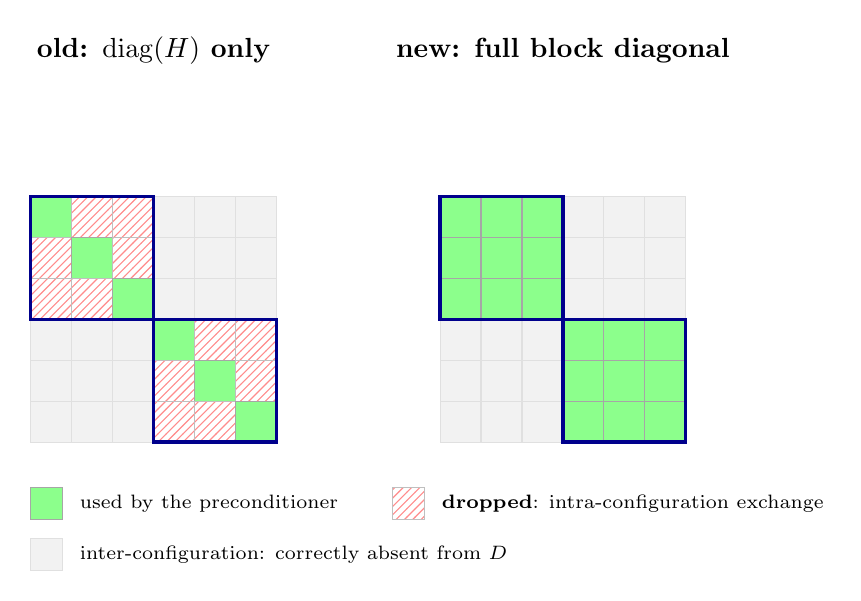
\begin{tikzpicture}[font=\small,scale=1.0]

  \def\cell{0.52}

  % ---------- left: what OLD uses ----------
  \begin{scope}[shift={(0,0)}]
    \node[font=\bfseries] at (1.56,1.85) {old: $\mathrm{diag}(H)$ only};
    \foreach \i in {0,1,2,3,4,5} {
      \foreach \j in {0,1,2,3,4,5} {
        \pgfmathtruncatemacro{\bi}{\i<3 ? 0 : 1}
        \pgfmathtruncatemacro{\bj}{\j<3 ? 0 : 1}
        \ifnum\bi=\bj
          \ifnum\i=\j
            \draw[fill=green!45,draw=black!35]
              (\j*\cell,-\i*\cell) rectangle ++(\cell,-\cell);
          \else
            \draw[fill=red!14,draw=black!25,pattern=north east lines,
                  pattern color=red!45]
              (\j*\cell,-\i*\cell) rectangle ++(\cell,-\cell);
          \fi
        \else
          \draw[fill=black!5,draw=black!12]
            (\j*\cell,-\i*\cell) rectangle ++(\cell,-\cell);
        \fi
      }
    }
    % block outlines
    \draw[very thick,blue!55!black] (0,0) rectangle (3*\cell,-3*\cell);
    \draw[very thick,blue!55!black] (3*\cell,-3*\cell) rectangle (6*\cell,-6*\cell);
  \end{scope}

  % ---------- right: what NEW uses ----------
  \begin{scope}[shift={(5.2,0)}]
    \node[font=\bfseries] at (1.56,1.85) {new: full block diagonal};
    \foreach \i in {0,1,2,3,4,5} {
      \foreach \j in {0,1,2,3,4,5} {
        \pgfmathtruncatemacro{\bi}{\i<3 ? 0 : 1}
        \pgfmathtruncatemacro{\bj}{\j<3 ? 0 : 1}
        \ifnum\bi=\bj
          \draw[fill=green!45,draw=black!35]
            (\j*\cell,-\i*\cell) rectangle ++(\cell,-\cell);
        \else
          \draw[fill=black!5,draw=black!12]
            (\j*\cell,-\i*\cell) rectangle ++(\cell,-\cell);
        \fi
      }
    }
    \draw[very thick,blue!55!black] (0,0) rectangle (3*\cell,-3*\cell);
    \draw[very thick,blue!55!black] (3*\cell,-3*\cell) rectangle (6*\cell,-6*\cell);
  \end{scope}

  % legend
  \begin{scope}[shift={(0,-4.1)},font=\scriptsize]
    \draw[fill=green!45,draw=black!35] (0,0) rectangle ++(0.4,0.4);
    \node[right] at (0.5,0.2) {used by the preconditioner};
    \draw[fill=red!14,draw=black!25,pattern=north east lines,pattern color=red!45]
      (4.6,0) rectangle ++(0.4,0.4);
    \node[right] at (5.1,0.2) {\textbf{dropped}: intra-configuration exchange};
    \draw[fill=black!5,draw=black!12] (0,-0.65) rectangle ++(0.4,0.4);
    \node[right] at (0.5,-0.45) {inter-configuration: correctly absent from $D$};
  \end{scope}

\end{tikzpicture}
\caption{The determinant--determinant Hamiltonian, restricted to two spatial
configurations (thick outlines). The old preconditioner used only the green
diagonal cells; the hatched off-diagonal cells inside each block --- the
exchange elements between determinants of the same configuration --- were
dropped. They are large and mostly negative, so the omission biases every
denominator in \eqref{eq:precond} the same way. Cells outside the blocks
belong to different configurations and are legitimately not part of a
\emph{block}-diagonal preconditioner.}
\label{fig:matrix}
\end{figure}

\subsection*{Why the symptom looked like it did}

Three observations that seemed puzzling all follow from one bias.

\paragraph{Spin stayed exact.}
$V$ is exact and fixed, so every trial vector is a target-$S$ combination no
matter what $D$ is. A bad preconditioner cannot contaminate the spin --- it
can only slow or stall the search. This is why the failure never presented as
spin contamination, and why the usual purification remedies would not have
helped.

\paragraph{Energies came out too high.}
With $D^{\text{old}} > D^{\text{new}}$ the denominators
$E^{(p)} - D_i$ are wrong in a consistent direction, so the correction vectors
are mis-scaled the same way at every iteration. The subspace stops making
progress on a plateau, and Davidson reports the best Ritz value it has found.
Since Ritz values are variational upper bounds, the result looks like a
legitimately converged energy that is simply too high --- there is no
error flag.

\paragraph{It got worse with $K$.}
At small $K$ the Krylov subspace grows to a sizeable fraction of the whole
space and reaches the true root regardless of preconditioning. As $K$ grows
that brute-force route disappears and the preconditioner quality becomes
decisive.

\medskip\noindent
This is precisely the ``spin-averaged preconditioner'' requirement of Fales,
Hohenstein and Levine (\emph{J.\ Chem.\ Theory Comput.}\ \textbf{13}, 4162
(2017), Sec.~2.6): a determinantal CI preconditioner must average the exchange
integrals \emph{within a spin-coupling set}. A \code{ConfigBlock} in
\code{single\_spin.h} \emph{is} one such set, and \eqref{eq:old} is exactly the
failure they warn about.

\section{The fix}

\subsection*{Exact block diagonal}

\code{build\_projected\_diagonal()} evaluates \eqref{eq:new} directly. For each
block it forms the small dense determinant--determinant submatrix $H_{bb}$ and
contracts it with the block's CSF coefficients. Diagonal entries are taken
from the precomputed \code{hii}; off-diagonal entries come from the general
\code{Hij(DetA,DetB,\dots)} primitive in
\code{chemistry/basic/determinants.h}, so SBD's own parity and phase
conventions are reused rather than reimplemented.

Cost is $O(\texttt{max\_block\_dim}\times N_{\text{det}})$ element
evaluations, once, before the iteration. Block dimensions are
$\binom{n_{\text{open}}}{n_{\uparrow}}$ and small in practice; at
$K=113\,394$ the whole setup measured $5.2\,$s against a $52\,$s solve.

\paragraph{A blind alley, recorded so it is not retried.}
An earlier attempt batched this extraction into \code{max\_block\_dim}
matrix--vector products, on the reasoning that blocks own disjoint determinant
index sets, so one probe vector set to $1$ on row $r$ of \emph{every} block
would yield that row for all blocks at once. This is wrong: $H$ couples
determinants of \emph{different} configurations, so each block's read-back is
contaminated by cross-block elements. A numerical check showed errors of the
same order as the matrix elements themselves. Direct \code{Hij} is both exact
and cheaper.

\subsection*{Seeding}

The seed was changed from the first $n_{\text{root}}$ unit CSF vectors
$e_0,\dots,e_{n_{\text{root}}-1}$ --- an arbitrary corner of the space, being
whichever configurations \code{std::map} happened to order first --- to the
$n_{\text{root}}$ unit vectors with the \emph{lowest} $D_c$. With the exact
$D$ these are the variationally best single-CSF starting guesses, and unit
vectors are trivially orthonormal so nothing extra is needed.

A useful side effect: the Rayleigh quotient of a single unit CSF vector
\emph{is} its own projected diagonal, so iteration \code{0.0} now prints an
energy equal to the reported seed \code{diag} value. That identity fails under
\eqref{eq:old}, which makes it a free per-run check that the exact diagonal is
in use.

\subsection*{Guard}

A configuration whose open-shell count has the wrong parity for the requested
$S_z$ is now skipped rather than silently truncating
$n_\uparrow = (n_{\text{open}} + 2S_z)/2$ by integer division.

\section{Effect}

\begin{table}[h]
\centering
\caption{Sampled N$_2$, $R=2.0$, 6-31G, 16 orbitals / 10 electrons, singlet,
3~roots, tolerance $10^{-8}$, 4~threads, stored-matrix path. Energies are
bit-identical before and after; only the iteration count changes.}
\label{tab:speed}
\begin{tabular}{lrrr}
\toprule
 & \multicolumn{2}{c}{inner steps} & \\
\cmidrule(lr){2-3}
$K$ & old & new & Davidson time (old\,$\to$\,new) \\
\midrule
$56$    & 31  & 21 & $0.0037 \to 0.0028$\,s \\
$117$   & 53  & 28 & $0.0071 \to 0.0042$\,s \\
$3\,906$ & 251 & 39 & $1.055 \to 0.196$\,s \quad(5.4$\times$) \\
\bottomrule
\end{tabular}
\end{table}

The speedup grows with $K$, which is the signature of a preconditioner problem
rather than a constant overhead. At $K=113\,394$ --- a case that previously
stalled or returned nonsense --- the solve now converges monotonically in
\textbf{25 matrix--vector products} over 2~restart cycles.

\begin{figure}[t]
\centering
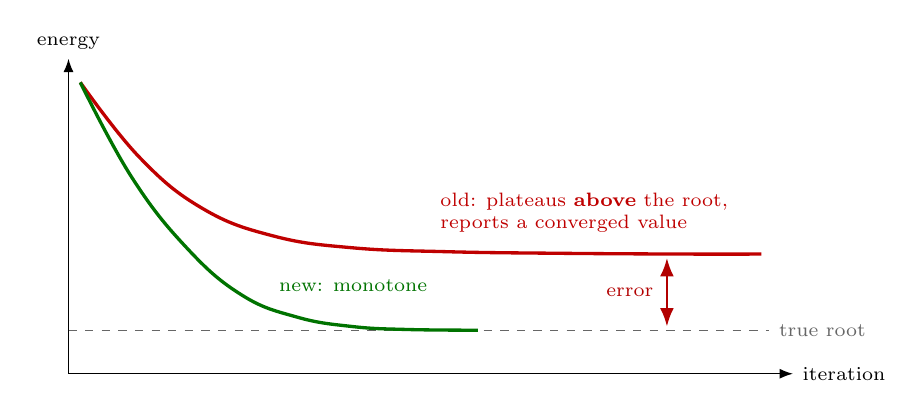
\begin{tikzpicture}[font=\small,>=Latex]
  \def\W{9.2}
  \def\Hh{4.0}

  % axes
  \draw[->] (0,0) -- (\W,0) node[right,font=\scriptsize] {iteration};
  \draw[->] (0,0) -- (0,\Hh) node[above,font=\scriptsize,align=center] {energy};

  % true root
  \draw[dashed,black!60] (0,0.55) -- (\W-0.3,0.55);
  \node[right,font=\scriptsize,black!60] at (\W-0.3,0.55) {true root};

  % OLD: descends then plateaus above the true root
  \draw[very thick,red!75!black]
    plot[smooth,tension=0.7] coordinates
    {(0.15,3.7) (0.9,2.75) (1.7,2.1) (2.6,1.75) (3.6,1.60) (4.8,1.55)
     (6.2,1.53) (7.8,1.52) (8.8,1.52)};
  \node[right,font=\scriptsize,red!75!black,align=left] at (4.6,2.05)
    {old: plateaus \textbf{above} the root,\\reports a converged value};

  % the gap
  \draw[<->,thick,red!70!black] (7.6,0.60) -- (7.6,1.47);
  \node[left,font=\scriptsize,red!70!black] at (7.55,1.04) {error};

  % NEW: monotone to the root
  \draw[very thick,green!45!black]
    plot[smooth,tension=0.7] coordinates
    {(0.15,3.7) (0.8,2.5) (1.5,1.6) (2.2,1.0) (2.9,0.72) (3.6,0.60)
     (4.3,0.562) (5.2,0.553)};
  \node[right,font=\scriptsize,green!45!black] at (2.55,1.12) {new: monotone};

\end{tikzpicture}
\caption{Schematic of the convergence behaviour (not measured data). The old
preconditioner biases every correction the same way, so the iteration settles
on a plateau above the true root and reports that value as converged; being a
Ritz value it is a legitimate variational upper bound, so nothing signals an
error. With the exact block diagonal the descent is monotone.}
\label{fig:convergence}
\end{figure}

\section{Verification}

\begin{itemize}\itemsep3pt
  \item \textbf{Formula.} The direct-\code{Hij} construction was checked
        against a brute-force $V^{\mathsf T} H V$ diagonal in double precision:
        agreement to $2\times10^{-16}$.
  \item \textbf{Energies.} An independent dense diagonalisation of $H$ and
        $\Sop^2$ over the same determinant list (built with the project's own
        Slater--Condon engine, outside SBD) reproduces the projected energies
        to all printed digits at $K=56$, $117$ and $3\,906$. At $K=3\,906$ the
        exact lowest singlets are $-108.792795252$, $-108.629192405$,
        $-108.588760240$, matching the solver.
  \item \textbf{Cross-checks at scale.} At $K=113\,394$ the Davidson energy,
        the explicit $\langle\psi|H|\psi\rangle$, and the trace of the
        one- plus two-body RDMs agree to ${\sim}10^{-13}$. The RDM route is
        independent of the solver path, so it also validates the
        CSF~$\to$~determinant rotation back.
  \item \textbf{Spin.} Converged roots are single-$S$ to machine precision, as
        they were before --- the fix does not touch spin purity, only the
        energy.
\end{itemize}

\paragraph{An interpretation trap worth flagging.}
In these sampled N$_2$ spaces at $K \le 3\,906$ the variational ground state
is a \emph{quintet} ($\langle \Sop^2\rangle = 6$), not a singlet. Single-spin
$E_0$ therefore correctly equals multi-spin $E_1$, and comparing it against
multi-spin $E_0$ makes a correct result look broken. The ordering is
size-dependent: at $K=113\,394$ the singlet \emph{is} lowest. Always compare
against the lowest multi-spin root with matching $\langle \Sop^2\rangle$.

\section{Where the code lives}

\begin{center}
\begin{tabular}{@{}ll@{}}
\toprule
\code{include/sbd/chemistry/gdb/single\_spin.h} & \\
\quad \code{build\_projected\_diagonal()} & exact $D$, Eq.~\eqref{eq:new} \\
\quad \code{\_davidson\_projected\_core()}  & uses $D$; falls back with a warning \\
\quad seeding block                         & lowest-$D$ unit vectors \\
\quad \code{build\_config\_projector()}     & $V$, plus the $S_z$ parity guard \\
\addlinespace
\code{include/sbd/chemistry/basic/determinants.h} & \\
\quad \code{Hij(DetA,DetB,\dots)}           & element primitive reused for $H_{bb}$ \\
\bottomrule
\end{tabular}
\end{center}

\noindent
The old approximation is retained as a fallback for callers that supply no
exact diagonal; it prints a warning that energies may converge above the true
root. Per-phase timings are available with \code{SBD\_SS\_TIMING=1}; note that
the printed \code{end davidson} interval brackets the projector build and the
per-root post-processing as well as the solve, so it is not the solve time
when \code{nroots > 1} and \code{--rdm 1}.

\end{document}
